%%
%% InterruptLab (c) 2021-23 Christopher A. Bohn
%%
%% Licensed under the Apache License, Version 2.0 (the "License");
%% you may not use this file except in compliance with the License.
%% You may obtain a copy of the License at
%%     http://www.apache.org/licenses/LICENSE-2.0
%% Unless required by applicable law or agreed to in writing, software
%% distributed under the License is distributed on an "AS IS" BASIS,
%% WITHOUT WARRANTIES OR CONDITIONS OF ANY KIND, either express or implied.
%% See the License for the specific language governing permissions and
%% limitations under the License.
%%

%%
%% (c) 2021 Christopher A. Bohn
%%

\documentclass[12pt]{article}

\usepackage{fullpage}
\usepackage{fancyhdr}
\usepackage[procnames]{listings}
\usepackage{hyperref}
\usepackage{textcomp}
\usepackage{bold-extra}
\usepackage[dvipsnames]{xcolor}
\usepackage{etoolbox}


% Customize the semester (or quarter) and the course number

\newcommand{\courseterm}{Spring 2022}
\newcommand{\coursenumber}{CSCE 231}

% Customize how a typical lab will be managed;
% you can always use \renewcommand for one-offs

\newcommand{\runtimeenvironment}{your account on the \textit{csce.unl.edu} Linux server}
\newcommand{\filesource}{Canvas or {\footnotesize$\sim$}cse231 on \textit{csce.unl.edu}}
\newcommand{\filesubmission}{Canvas}

% These are placeholder commands and will be renewed in each lab

\newcommand{\labnumber}{}
\newcommand{\labname}{Lab \labnumber\ Assignment}
\newcommand{\shortlabname}{}
\newcommand{\duedate}{}

% Individual or team effort

\newcommand{\individualeffort}{This is an individual-effort project. You may discuss concepts and syntax with other students, but you may discuss solutions only with the professor and the TAs. Sharing code with or copying code from another student or the internet is prohibited.}
\newcommand{\teameffort}{This is a team-effort project. You may discuss concepts and syntax with other students, but you may discuss solutions only with your assigned partner(s), the professor, and the TAs. Sharing code with or copying code from a student who is not on your team, or from the internet, is prohibited.}
\newcommand{\freecollaboration}{In addition to the professor and the TAs, you may freely seek help on this assignment from other students.}
\newcommand{\collaborationrules}{}

% Do you care about software engineering?

\providebool{allowspaghetticode}

\setbool{allowspaghetticode}{false}

\newcommand{\softwareengineeringfrontmatter}{
    \ifboolexpe{not bool{allowspaghetticode}}{
        \section*{No Spaghetti Code Allowed}
        In the interest of keeping your code readable, you may \textit{not} use
        any \lstinline{goto} statements, nor may you use any \lstinline{break}
        statements to exit from a loop, nor may you have any functions
        \lstinline{return} from within a loop.
    }{}
}

\newcommand{\spaghetticodepenalties}[1]{
    \ifboolexpe{not bool{allowspaghetticode}}{
        \penaltyitem{1}{for each \lstinline{goto} statement, \lstinline{break}
            statement used to exit from a loop, or \lstinline{return} statement
            that occurs within a loop.}
    }{}
}

% You shouldn't need to customize these,
% but you can if you like

\lstset{language=C, tabsize=4, upquote=true, basicstyle=\ttfamily}
\newcommand{\function}[1]{\textbf{\lstinline{#1}}}
\setlength{\headsep}{0.7cm}
\hypersetup{colorlinks=true}

\newcommand{\startdocument}{
    \pagestyle{fancy}
    \fancyhf{}
    \lhead{\coursenumber}
    \chead{\ Lab \labnumber: \labname}
    \rhead{\courseterm}
    \cfoot{\shortlabname-\thepage}

	\begin{document}
	\title{\ Lab \labnumber}
	\author{\labname}
	\date{Due: \duedate}
	\maketitle

    \textit{\collaborationrules}
}

\newcommand{\rubricitem}[2]{\item[\underline{\hspace{1cm}} +#1] #2}
\newcommand{\bonusitem}[2]{\item[\underline{\hspace{1cm}} Bonus +#1] #2}
\newcommand{\penaltyitem}[2]{\item[\underline{\hspace{1cm}} -#1] #2}

%%
%% labs/common/semester.tex
%% (c) 2021-22 Christopher A. Bohn
%%
%% Licensed under the Apache License, Version 2.0 (the "License");
%% you may not use this file except in compliance with the License.
%% You may obtain a copy of the License at
%%     http://www.apache.org/licenses/LICENSE-2.0
%% Unless required by applicable law or agreed to in writing, software
%% distributed under the License is distributed on an "AS IS" BASIS,
%% WITHOUT WARRANTIES OR CONDITIONS OF ANY KIND, either express or implied.
%% See the License for the specific language governing permissions and
%% limitations under the License.
%%


% Customize the semester (or quarter) and the course number

\newcommand{\courseterm}{Fall 2022}
\newcommand{\coursenumber}{CSCE 231}

% Customize how a typical lab will be managed;
% you can always use \renewcommand for one-offs

\newcommand{\runtimeenvironment}{your account on the \textit{csce.unl.edu} Linux server}
\newcommand{\filesource}{Canvas or {\footnotesize$\sim$}cse231 on \textit{csce.unl.edu}}
\newcommand{\filesubmission}{Canvas}

% Customize for the I/O lab hardware

\newcommand{\developmentboard}{Arduino Nano}
%\newcommand{\serialprotocol}{SPI}
\newcommand{\serialprotocol}{I2C}
%\newcommand{\displaymodule}{MAX7219digits}
%\newcommand{\displaymodule}{MAX7219matrix}
\newcommand{\displaymodule}{LCD1602}

\setbool{usedisplayfont}{true}

\newcommand{\obtaininghardware}{
    The EE Shop has prepared ``class kits'' for CSCE 231; your class kit costs \$30.
    The EE Shop is located at 122 Scott Engineering Center and is open M-F 7am-4pm. You do not need an appointment.
    You may pay at the window with cash, with a personal check, or with your NCard.
    The EE shop does \textit{not} accept credit cards.
}

% Update to reflect the CS2 course(s) at your institute

\newcommand{\cstwo}{CSCE~156, RAIK~184H, or SOFT~161}

% Do you care about software engineering?

\setbool{allowspaghetticode}{false}

% Which assignments are you using this semester, and when are they due?

\newcommand{\pokerlabnumber}{1}
\newcommand{\pokerlabcollaboration}{
    Sections~\ref{sec:connecting}, \ref{sec:terminology}, \ref{sec:gettingstarted}, \ref{subsec:typesofpokerhands}, and~\ref{subsec:studythecode}: \freecollaboration
    Sections~\ref{sec:completingcard} and~\ref{subsec:completepoker}: \individualeffort
}
\newcommand{\pokerlabdue}{Week of August 29, before the start of your lab section}

\newcommand{\keyboardlabnumber}{2}
\newcommand{\keyboardlabcollaboration}{\individualeffort}
\newcommand{\keyboardlabdue}{Week of January 31, before the start of your lab section}

\newcommand{\pointerlabnumber}{3}
\newcommand{\pointerlabcollaboration}{\individualeffort}
\newcommand{\pointerlabdue}{Week of February 7, before the start of your lab section}

\newcommand{\integerlabnumber}{4}
\newcommand{\integerlabcollaboration}{\individualeffort}
\newcommand{\integerlabdue}{Week of February 14, before the start of your lab section}

\newcommand{\floatlabnumber}{5}
\newcommand{\floatlabcollaboration}{\individualeffort}
\newcommand{\floatlabdue}{soon}

\newcommand{\addressinglabnumber}{6}
\newcommand{\addressinglabcollaboration}{\individualeffort}
\newcommand{\addressinglabdue}{Week of February 28, before the start of your lab section}

%bomblab was 7
%attacklab was 8

\newcommand{\pollinglabnumber}{9}
\newcommand{\pollinglabcollaboration}{\individualeffort}
\newcommand{\pollinglabdue}{Week of April 11, before the start of your lab section}
\newcommand{\pollinglabenvironment}{your \developmentboard-based class hardware kit}

\newcommand{\ioprelabnumber}{\pollinglabnumber-prelab}
\newcommand{\ioprelabcollaboration}{\freecollaboration}
\newcommand{\ioprelabdue}{Before the start of your lab section on April 5 or 6}

\newcommand{\interruptlabnumber}{10}
\newcommand{\interruptlabcollaboration}{\individualeffort}
\newcommand{\interruptlabdue}{Week of April 18, before the start of your lab section}
\newcommand{\interruptlabenvironment}{your \developmentboard-based class hardware kit}

\newcommand{\capstonelab}{ComboLock}    % this will come into play when we generalize capstonelab
\newcommand{\capstonelabnumber}{11}
\newcommand{\capstonelabcollaboration}{\teameffort}
\newcommand{\capstonelabdue}{Week of May 2, Before the start of your lab section\footnote{See Piazza for the due dates of teams with students from different lab sections.}}
\newcommand{\capstonelabenvironment}{your \developmentboard-based class hardware kit}

\newcommand{\memorylabnumber}{12}
\newcommand{\memorylabcollaboration}{This is an individual-effort project. You may discuss the nature of memory technologies and of memory hierarchies with classmates, but you must draw your own conclusions.}
\newcommand{\memorylabdue}{Week of May 2, at the end of your lab section}
\newcommand{\memorylabenvironment}{your \developmentboard-based class hardware kit and your account on the \textit{csce.unl.edu} Linux server}

% Labs not used this semester

\newcommand{\concurrencylabnumber}{XX}
\newcommand{\concurrencylabcollaboration}{\individualeffort}
\newcommand{\concurrencylabdue}{not this semester}

\newcommand{\ssbcwarmupnumber}{XX}
\newcommand{\ssbcwarmupcollaboration}{\freecollaboration}
\newcommand{\ssbcwarmupdue}{not this semester}

\newcommand{\ssbcpollingnumber}{XX}
\newcommand{\ssbcpollingcollaboration}{\individualeffort}
\newcommand{\ssbcpollingdue}{not this semester}

\newcommand{\ssbcinterruptnumber}{XX}
\newcommand{\ssbcinterruptcollaboration}{\individualeffort}
\newcommand{\ssbcinterruptdue}{not this semester}

%%
%% labs/common/storylines.tex
%% (c) 2020-23 Christopher A. Bohn
%%
%% Licensed under the Apache License, Version 2.0 (the "License");
%% you may not use this file except in compliance with the License.
%% You may obtain a copy of the License at
%%     http://www.apache.org/licenses/LICENSE-2.0
%% Unless required by applicable law or agreed to in writing, software
%% distributed under the License is distributed on an "AS IS" BASIS,
%% WITHOUT WARRANTIES OR CONDITIONS OF ANY KIND, either express or implied.
%% See the License for the specific language governing permissions and
%% limitations under the License.
%%

\newcommand{\MeetArchie}{
    \begin{wrapfigure}{r}{0.33\textwidth}
        \centering
        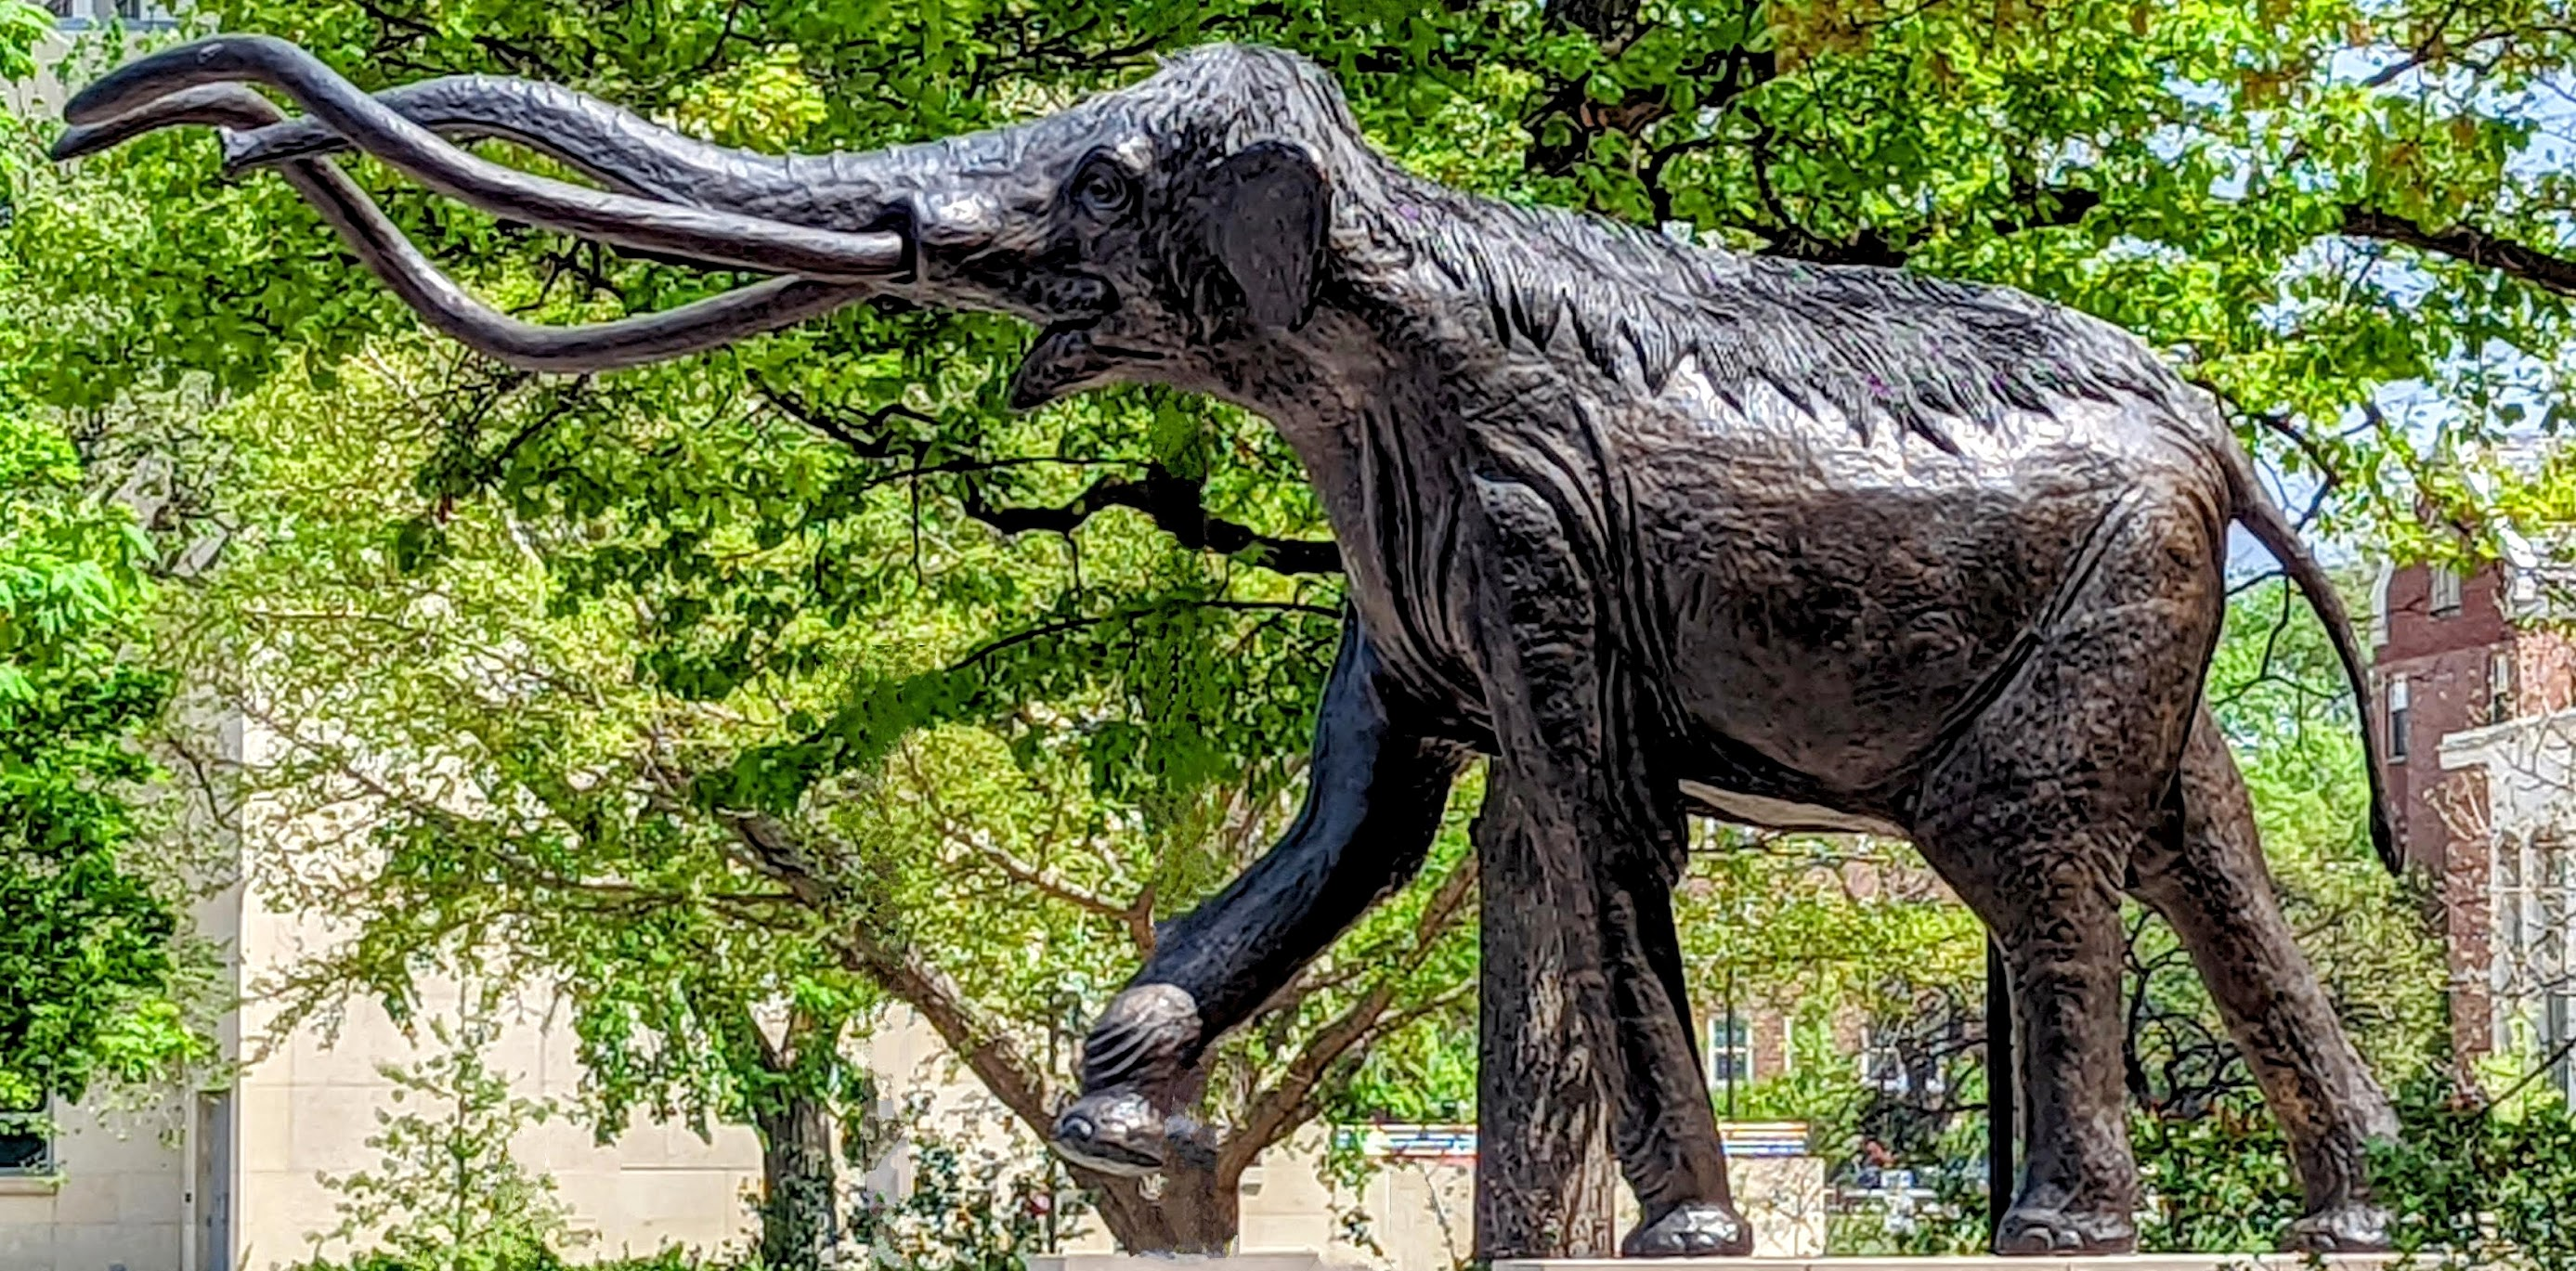
\includegraphics[width=.4\textwidth]{archie}
        \caption{Archie.\\ \footnotesize{Photograph by Bohn.}}
    \end{wrapfigure}

    You're relaxing at your favorite hangout when another customer catches your attention.
    He's rather large (dare I say, \textit{mammoth}), a bit hairy, and looking frustrated in front of his laptop.
    ``I'm Archie,'' he says, ``and I'm trying to teach myself this card game called \textit{Poker}.
    I found this source code that I thought I could use to understand Poker better, but the code is incomplete, and I don't entirely understand what's there.
    Could you explain the code to me, please?'
}

\newcommand{\GetHired}{
    Archie's face lights up in a very big smile.
    ``Thanks!''
    After pausing in thought for a moment, he says, ``Say, I've got a new startup company that could really use your help.
    Are you interested?
    It'll be exciting!''
}

\newcommand{\FirstDayOnTheJob}{
    \begin{wrapfigure}{r}{0.33\textwidth}
        \centering
        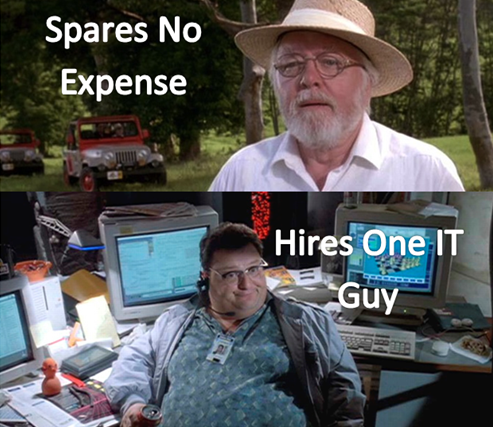
\includegraphics[width=.4\textwidth]{some-expenses-spared}
        \caption{Some expenses were spared.\\ \footnotesize{Original images \textcopyright\ Universal Studios and Amblin Entertainment, Inc. Meme creator unknown.}}
    \end{wrapfigure}

    You've recently been hired to help get the Pleistocene Petting Zoo get started.
    Your new employer, Archie, is surprisingly honest: he admits to you that some expenses were spared.
    Archie cheerfully points out that any challenge is also an opportunity to succeed.
    You suspect your job will offer plenty of ``opportunities to succeed.''
}

\newcommand{\HasKeyboard}{
    Great news!
    Archie brings you your new keyboard.
    He also brings you a problem of his own.
    Because you were held up with the broken keyboard, Archie decided to try some programming on his own, and his code is behaving strangely.
}

\newcommand{\ArchieWroteSmellyCode}{
    Working at the Pleistocene Petting Zoo certainly is proving to be interesting.
    You're glad that you don't have to worry about the problem of the giant sloths very slowly chasing their handlers, but now it seems that Archie has decided to try to write a program or two.
    At a glance, his code is smellier than the wooly rhinoceros' enclosure.
    But you take a closer look anyway to try to understand why his code acts strangely.
}

\newcommand{\InsurancePreview}{
    You hear somebody enter the room.
    ``\textit{Frankenstein}, `boat','' is the challenge, and she answers, ``borne.''
    Archie introduces you to the new arrival, ``Lil, this is our new developer, the one who wrote the app we just used.''
    He turns to you: ``This is Lilith Redd from business operations.''
    He turns back to her and continues, ``Lil, what's the good word?''

    ``The word isn't good, I'm afraid.
    I just heard back from the insurance company.''
}

\newcommand{\OnLoanToEclecticElectronics}{
    All work at the Pleistocene Petting Zoo has stopped while Archie tries to find a $\cancelto{\mathrm{reasonable}}{\mathrm{gullible}}$ insurance company.
    Rather than furloughing staff, he's asked everybody to help out with his other startup companies for a week or two.
    He specifically asked that you help out with Eclectic Electronics.

    Herb Bee, the chief engineer, explains that Eclectic Electronics is developing a patent-pending C-licon tool that will convert C code into an integrated circuit that has the same functionality as the original C code.
    To test it out, he tasked you with writing the code to implement an Arithmetic Logic Unit (ALU).
    Your task will be to implement integer addition, subtraction, multiplication, and division.
    Even though high-level languages' \textit{logical} boolean operations normally are not part of an ALU, Herb wants you to include these in the ALU to see if that can make some programs run faster.
    Because bitwise operations and bit shift operations have been implemented, you will be able to use C's bitwise and bit shift operators, but because arithmetic operations have not yet been implemented, you cannot use C's arithmetic operators.
    Because C library functions generally make use of arithmetic operations (which have not yet been implemented), you cannot use library functions.
}

\newcommand{\SuccessfulALU}{
    Herb smiles as he hands you the the test results from the latest integrated circuit fab batch.
    ``C-licon successfully turned your code into an ALU.
    Nicely done!''
    I think maybe it's time to use C-licon to see if we can improve the Floating Point Unit (FPU) on our experimental microprocessor.
}

\newcommand{\WriteAnFPU}{
    Herb tells you that, Eclectic Electronics tested the integrated circuit that the C-licon tool created from your ALU code, and they've concluded that C-licon is ready to use for their new experimental microprocessor.
    He tasks you with writing C code (that will be used by the C-licon tool) to implement a Floating Point Unit (FPU).
    Your task will be to implement floating point addition, subtraction, multiplication, and division.
    You can use any bit operations and, thanks to the ALU you wrote, you can use any integer arithmetic operations (use the conventional + - * / operators).
    Because the FPU has not yet been implemented, you cannot use C's floating point operations, you cannot use \lstinline{float}s nor \lstinline{double}s, and you cannot use library functions.
}

\newcommand{\GoingBackToTheZoo}{
    Lil enters the room.
    Herb challenges her: ``\textit{Gulliver's Travels}, `endian','' and Lil answers, ``ends.''

    Lil walks up to you and says, ``We have the insurance situation taken care of, and it's time to get the Zoo ready for guests.
    We're reassembling the tech team, and there's plenty of work to do.''

    You smile.
    ``That's good news!''

    Lil's face is hard to read.
    ``Well, yes and no.
    It's good that you'll be able to resume work on the Zoo's systems.
    But while Archie was waiting for us to fix the insurance situation, he got bored and -- cutting a long story short -- he ended up creating some new `opportunities' that we need you `to succeed' at.''
}

\newcommand{\SettledIntoRoutine}{
    You've settled into a comfortable routine at the Pleistocene Petting Zoo.
    While your job isn't quite as exciting as that of the saber-toothed tigers' dentist, it still has something new and interesting almost every day.

    Archie announces that he heard that hand-crafted assembly code can be faster than high-level language code.
    You try to explain that while this may have been true decades ago, modern optimizing compilers generate code faster than what a typical programmer can achieve with assembly code.
    Archie doesn't believe you and insists that you write the zoo's new cipher program in x86 assembly code.
}

\newcommand{\NewmanRanOffWithSamples}{
    Archie is hurriedly packing is trunk, like he's about to leave on a short-notice urgent trip.
    Before charging out the door, he pauses to tell you, ``Newman just stole some of our samples.
    I need to track him down before he sells them to the Supersized Safari Syndicate.
    I guess this means you're in charge of the Zoo's computer system now.
    Don't worry, you'll be fine. What could possibly go wrong?''
}

\newcommand{\BombLabIntroduction}{  % Ties Bryant & O'Halloran's Bomb Lab into the Pleistocene Petting Zoo story
    In a jarring collision of movie franchises, the CEO of Virtucon makes a Zoom call to the Pleistocene Petting Zoo.
    For some reason that nobody really explains, you're the only person available to handle the situation.
    The guy, who sounds kind of like an animated ogre, demands that the Pleistocene Petting Zoo deliver to him a megalodon shark with a head-mounted laser capable of emitting a beam of pure antimatter.

    You blurt out, ``Then it's not a laser,'' and then try to explain to him that megalodons are from the Miocene epoch, and expecting to find them at the Pleistocene Petting Zoo would be as ridiculous as a Cretaceous-period tyrannosaur at a Jurassic-themed park.

    ``Zip it!'' commands the guy who kind of looks like the host of a public-access show you used to watch.
    ``Since you won't meet my demand, my minions have placed a `binary bomb' under your zoo.
    Because I like really convoluted plans, we put software on your Linux server that controls the bomb.
    If you do nothing, the bomb will explode.
    If you turn off the Linux server, the bomb will explode.
    If you go slower than 50mph, the bomb will -- no, never mind that last part.

    ``The bomb software consists of a sequence of phases.
    Each phase expects you to type a particular string on \texttt{stdin}.
    If you type the correct string, then the phase is {\em defused} and the bomb proceeds to the next phase. Otherwise, the bomb {\em explodes}.
    The bomb is defused when every phase has been defused.

    ``Your mission, which you have no choice but to accept, is to defuse your bomb before the due date.
    Good luck, and welcome to the bomb squad!''
}

\newcommand{\FoodLockersAreStuck}{
    Having saved the Zoo from Dr. Evil's binary bomb, you relax back in your chair and think about taking a break.
%SPRINGBREAK
    Maybe an entire week in which you don't have solve any problems or meet any deadlines -- that'd be real nice.
%FALLBREAK
    % Maybe 4-day weekend in which you don't have solve any problems or meet any deadlines -- that'd be real nice.

    Another Zoom call comes in.
    \textit{What now!?} you wonder as you take your feet off of the desk to answer the call.
    An uncomfortable-looking animal handler says, ``We can't unlock the food lockers.
    It's the animals' feeding time, and we can't open the food lockers!
    It's feeding time, we can't get to the animals' food, and,'' his eyes dart nervously toward the animal enclosures, ``and many of them have sharp, pointy claws and others have big, stompy feet.''
}

\newcommand{\AttackLabIntroduction}{    % Ties Bryant & O'Halloran's Attack Lab into the Pleistocene Petting Zoo story
    You managed to keep the Pleistocene Petting Zoo from blowing to smithereens, but it turns out that Dr. Evil's minions weren't too careful when they put the bomb control software on the Zoo's Linux server.
    The software that controls the food locker has been heavily damaged!
    The functions that unlock the food locker doors are still present, but there's no way to activate those functions.

    You then recall what Archie told you when he hired you: some expenses were spared.
    You run the machine code through a disassembler and quickly see that it has a buffer overflow vulnerability.
    Before the situation in the dire wolf enclosure gets too dire, you sit down and get to work.

    The \function{ctarget} code runs on an older machine that allows executable code to be present on the stack, so it's vulnerable to a conventional code injection buffer overflow attack.
    \begin{itemize}
        \item Phase 1 (\function{touch1}) unlocks the food locker so the animal handlers can prepare the food.
        \item Phase 2 (\function{touch2}) opens the doors between the food locker and the carnivore enclosures;
        you will need to pass a cookie to the function to authenticate yourself.
        \item Phase 3 (\function{touch3}) closes the doors between the food locker and the carnivore enclosures.
    \end{itemize}
    The \function{rtarget} code runs on a newer machine that does not allow executable code to be present on the stack, so you'll have to conduct a return-oriented programming attack on it.
    \begin{itemize}
        \item Phase 4 (\function{touch2)} opens the doors between the food locker and the herbivore enclosures;
        you will need to pass a cookie to the function to authenticate yourself.
        \item Phase 5 (\function{touch3}) closes the doors between the food locker and the herbivore enclosures.
    \end{itemize}
}

\newcommand{\MostAnimalsAreFed}{
    Before you take on the Phase 5, pause to consider what you have accomplished so far.
    In Phases 2 and 3, you caused a program to execute machine code of your own design.
    If {\sc ctarget} had been a network server, you could have injected your own code into a distant machine.
    In Phase 4, you circumvented two of the main devices modern systems use to thwart buffer overflow attacks.
    Although you did not inject your own code, you were able inject a type of program that operates by stitching together sequences of existing code.
    Also, all animals have been fed, the carnivores are still in their enclosure, the mammoths can't fit through the herbivore door, and only the giant sloths seem interested in very slowly escaping.
}

\newcommand{\ArchieReturns}{
    Archie returns from tracking down Newman, who'd run off with some of the Pleistocene Petting Zoo's samples shortly before Dr.~Evil's Zoom call.
    ``It turns out he didn't get very far at all,'' Archie sighs.
    ``He ran into a flock of terror birds as he was leaving, and we found him in one of the emergency shelters.

    Archie smiles. ``I trust things were uneventful while I was away?''
}

\newcommand{\PickingUpNewmansProject}{
    Archie seems genuinely surprised that Newman is refusing to go back to work.
    ``You would think that he'd be grateful for being rescued from that flock of terror birds.''
    Before you can wonder out-loud whether it would be a good idea to trust someone who had just tried to sell trade secrets to a competitor, Archie gives you your new task.

    ``Because Newman isn't cooperating, I need you to finish the project he was working on.
    As you can imagine, duplicating the genetic information for our exhibits can take a long time, and Newman realized that we might be able to duplicate the data faster if we had a concurrent program which has one thread reading from the original data and another thread writing the copy.
    Unfortunately, he ran off to sell samples to the  Supersized Safari Syndicate before finishing the duplicator.
    Right now the duplicator seems to work, but it usually makes imperfect copies.
    Have you ever seen a paleolama with two noses, four eyes, and no ears!?''
}

\newcommand{\WeNeedBetterDetection}{
    Between Newman trying to sell samples to a competitor, that weird guy almost blowing up the zoo, and the animals almost escaping, Archie is getting worried.
    ``I think we need to introduce additional protective measures.
    As useful as your challenge-response app is in helping us detect intruders, I think it's now clear that we need something that will detect someone -- or some\textit{thing} -- when they're someplace they shouldn't be, even when no one else is around.
    I've asked the team at Eclectic Electronics to put something together.''
}

\newcommand{\WeNeedBetterLocks}{
    Between Newman trying to sell samples to a competitor, that weird guy almost blowing up the zoo, and the animals almost escaping, Archie is getting worried.
    ``I think we need to introduce additional protective measures.
    As useful as your challenge-response app is in helping us detect intruders, I think it's now clear that we need something that will keep someone -- or some\textit{thing} -- out of places they shouldn't be, even when no one else is around.
    I've asked the team at Eclectic Electronics to put something together.''
}

\newcommand{\IntroduceHardware}{
    Archie walks up to you, along with Herb Bee from Eclectic Electronics.
    Herb is holding a tangled mess of electronics.
    Archie explains, ``Herb here has developed a prototype of a device that he thinks will be useful for our physical security needs, as well as a few other applications around here. He calls it the \textit{Cow Pi}.''

% TODO: parameterize based on which microcontroller is actually being used
    You look at the device in Herb's hands and see the \nano\ central to the circuit.
    ``Isn't \textit{-Pi} typically used as a suffix for circuits that use a Raspberry Pi instead of an Arduino?''

    Herb replies, ``Typically, yes, but \textit{Cowduino} isn't very punny, is it?''

    Archie chimes in, ``Maybe with the right emphasis: \textit{Cow-DOO-ino}.''

    ``That's kind of subtle, don't you think? How will people know to put the emPHAsis on that sylLAble?''

    ``I think we're getting off topic here,'' you point out.
    ``How can I help?''

    ``Oh, right,'' Herb says, ``We'd like you to kick its proverbial tires.
    Let's start off with something simple, like a number builder tool.''
}

\newcommand{\JeffGoldblum}{
    Herb looks over your work.
    ``Hmm, yes. I think this is coming along nicely.
    Let's run a few more tests.''

    Archie storms into the room.
    ``We have \textit{got} to do something about security!
    How's that doodad coming along?
    Because there's now a half-man/half-fly in the labs going on-and-on about Chaos Theory and how if we just give him a MacBook and a spaceship then he'll be able to get the Lord of Thunder to travel across the 8th Dimension.
    Is that thing just about ready?''

    Herb shakes his head, ``No, not quite yet. It should be ready in about a week.''
}

\newcommand{\DisdainfulHerb}{
    Smoke wafts from Herb's soldering iron as he looks up when you approach.
    Cleaning the iron's tip, he quotes:
    ``Somebody once said, `The three most dangerous things in the world are a programmer with a soldering iron, a hardware engineer with a software patch, and'{}'' -- he glances nervously in Archie's direction -- ``{}`a user with an idea.'\footnote{
        Rick Cook, \textit{The Wizardry Consulted}, 1995.
    }$^{\mathrm{,}}$\footnote{
        The notion of being wary of programmers wielding screwdrivers or soldering irons long pre-dated this quote, as there are apocryphal tales of people who found it easier to modify the hardware to suit the software rather than the other way around.
    }''
}

\newcommand{\NumberConversionTool}{     % Since we're now allowing `sprintf()` with the LCD1602, converting between decimal and hexadecimal is trivial; it still might be okay for 7-segment displays
    Herb gets straight to the point.
    ``We promised Archie that we'd be able to start using the Cow Pi to build systems in a week.
    So far we've tested its input/output functionality, but we still need to test its timer and also whether we can take inputs without constantly polling the input devices.
    As before, we don't need to do anything too fancy;
    let's try a number base conversion tool.''
}

\newcommand{\LessDisdainfulHerb}{
    Smoke wafts from Herb's soldering iron as he looks up when you approach.
    Cleaning the iron's tip, he notes:
    ``Somebody once said that one of the most dangerous things in the world is a programmer with a soldering iron.''\footnote{
        ``The three most dangerous things in the world are a programmer with a soldering iron, a hardware engineer with a software patch, and a user with an idea.'' -- Rick Cook, \textit{The Wizardry Consulted}, 1995.
    }$^{\mathrm{,}}$\footnote{
        The notion of being wary of programmers wielding screwdrivers or soldering irons long pre-dated this quote, as there are apocryphal tales of people who found it easier to modify the hardware to suit the software rather than the other way around.
    }
}

\newcommand{\RemoteControlledCar}{

    About this time, Archie walks by, thinking about electric carts to transport visitors around the Pleistocene Petting Zoo.
    ``They probably should be remote-controlled.''
    He looks at you and Herb, and asks, ``Do you think you could make a cart a remote-controlled cart?''

    You ask the obvious question, ``Are there carts here already?''

    Archie waves his hand in the air, dismissing that detail, ``Not yet, but could you make the remote-control?''
    
    You hestatingly summarize: ``You want a cartless remote-controlled cart?''

    Archie beamingly smiles, ``Exactly!''

    Herb jumps in, ``Yes, we'll do it.''
    Herb looks at you and adds, ``It'll give us a chance to test the Cow Pi's timer and whether we can take inputs without constantly polling the input devices.''
}

\newcommand{\LauraDern}{
    You and Herb look for Archie in the Pleistocene Petting Zoo's labs to give him the good news, and you find a blond woman wearing cargo shorts, butchering a Gilbert and Sullivan song\dots \\ \\
    \textmusicalnote\ I am the very model of a modern vice admiral \textmusicalnote \\
    \textmusicalnote\ I've information about all things paleobotanical \textmusicalnote \\
    \textmusicalnote\ And I've been up to my armpits in problems scatological \textmusicalnote \\
    \textmusicalnote\ During the regency I had experience matriarchical \textmusicalnote \\
    \textmusicalnote\ I plot space travel, normal and superluminal \textmusicalnote \\
    \textmusicalnote\ (Even if I challenge the Pauli exclusion principle) \textmusicalnote \\

    ``I don't know how these people keep getting into our labs.
    \textit{Please} tell me that you have good news,'' pleads Archie.

    ``Yes, the Cow Pi is ready for whatever you need: calculators, security systems, parking meters -- you name it,'' Herb cheerfully responds.

    ``Excellent.''
    Archie turns to you.
    ``I'd like you and Newm... no, \textit{not} Newman.
    I'd like you and someone else on the staff to get started right away.
    Here's what I'd like to have built first.''
}

\newcommand{\CalculatorNeeded}{
    ``I have various teams working on different projects around here to improve security,'' Archie reminds you.
    He glances toward the Zoo's labs, where there's now a guy who looks like the actor who portrayed the fictional actor who portrayed the Norse god Odin, trying to avoid children while wistfully talking about raising rabbits in Montana.
    You briefly wonder why there are children someplace where there are also carnivorous megafauna, and then you remember that you work at a petting zoo.
    ``What I need your team to do,'' Archie continues, ``is make a four-function calculator so that we can quickly and easily determine whether we have the correct number of specimens, or if any are missing.''
}

\newcommand{\CalculatorCounting}{
    Technicians are using your calculator to compute how many specimens are still present in the lab, and establish that all specimens are accounted for after Newman's attempted theft.
    As reports come in of facilities getting secured with Cow Pi-based locks and passages being monitored with Cow Pi-based motion sensors, Archie smiles and tells you that this was a job well done.
    With all of the excitement neatly wrapped-up and arriving at a satisfactory conclusion, you look forward to a boring career in which there's absolutely no screaming and running for your life.
}

\newcommand{\CombinationLockNeeded}{
    ``I have various teams working on different projects around here to improve security,'' Archie reminds you.
    He glances toward the Zoo's labs, where there's now a guy who looks like the actor who portrayed the fictional actor who portrayed the Norse god Odin, trying to avoid children while wistfully talking about raising rabbits in Montana.
    You briefly wonder why there are children someplace where there are also carnivorous megafauna, and then you remember that you work at a petting zoo.
    ``What I need your team to do,'' Archie continues, ``is make a combination lock so that only authorized people can get into our lab facilities.''
}

\newcommand{\CombinationLockInstalled}{
    After fastening the new electronic combination lock to the lab door, Archie smiles and tells you that this was a job well done.
    With all of the excitement neatly wrapped-up and arriving at a satisfactory conclusion, you look forward to a boring career in which there's absolutely no screaming and running for your life.
}

\newcommand{\RangeFinderNeeded}{
    ``I have various teams working on different projects around here to improve security,'' Archie reminds you.
    He glances toward the Zoo's labs, where there's now a guy who looks like the actor who portrayed the fictional actor who portrayed the Norse god Odin, trying to avoid children while wistfully talking about raising rabbits in Montana.
    You briefly wonder why there are children someplace where there are also carnivorous megafauna, and then you remember that you work at a petting zoo.
    ``What I need your team to do,'' Archie continues, ``is make a range finder that will alert us when someone -- or some\textit{thing} -- gets too close to someplace they shouldn't be.''
}

\newcommand{\RangeFinderDetecting} {
    A technician installing a new range finder outside the lab door briefly sets off the alarm, but then the range finder falls quiet and faithfully reports that nothing is approaching.
    As reports come in of facilities getting secured with Cow Pi-based locks, and of accurate speciment counts accomplished with Cow Pi-based calculators, Archie smiles and tells you that this was a job well done.
    With all of the excitement neatly wrapped-up and arriving at a satisfactory conclusion, you look forward to a boring career in which there's absolutely no screaming and running for your life.
}

\usepackage{amsmath}
%\usepackage{array,color,colortbl}
\definecolor{LightGreen}{rgb}{0.88,1,0.88}
\usepackage{multicol}
\usepackage{CJKutf8}
\usepackage{gensymb}
\setlength{\columnsep}{2cm}


% \captionsetup{width=.8\linewidth}

% \lstset{language=c, numbers=left, showstringspaces=false,
%     moredelim = [s][\ttfamily]{/*}{*/} % I shouldn't need this parameter!
%     }

\renewcommand{\labnumber}{\interruptlabnumber}
\renewcommand{\labname}{Using Interrupt-Driven Input/Output}
\renewcommand{\shortlabname}{interrupt-driven i/o -- interruptlab}
\renewcommand{\collaborationrules}{\interruptlabcollaboration}
\renewcommand{\duedate}{\interruptlabdue}
\newcommand{\nano}{\developmentboard} % TODO: replace \nano with \developmentboard
\renewcommand{\runtimeenvironment}{\interruptlabenvironment}
\pagelayout
\begin{document}
    \labidentifier

    \pdfbookmark[1]{Frontmatter}{frontmatter}                                       In this assignment, you will write code for \runtimeenvironment\ that will use new electronic devices to interact with the physical world.

The instructions are written assuming you will edit the code in the Arduino IDE and run it on \runtimeenvironment, constructed according to the pre-lab instructions.
If you wish, you may edit the code in a different environment; however, our ability to provide support for problems with other IDEs is limited.

\section*{Learning Objectives}

After successful completion of this assignment, students will be able to:
\begin{itemize}
    \item Work collaboratively on a hardware/software project
    \item Design and implement a simple embedded system
    \item Expand their programming knowledge by consulting documentation
\end{itemize}

\subsection*{Continuing Forward}

This penultimate lab assignment does not contribute to the final lab assignment.
By integrating elements of what you learned in this course, and by demonstrating that you can review documentation to learn on your own, to design a small embedded system, you will show how much progress you have made this semester.

\section*{During Lab Time}

During your lab period, coordinate with your group partner(s) to decide on your working arrangements.
Unless you're only going to work on the assignment when you're together, you may want to set up a private Git repository that is shared with your partner(s).
With your partner(s), modify your hardware kit as described in Section~\ref{sec:hardwareMods}.
Then, think through your system's design and begin implementing it.
The TAs will be available for questions.


    \softwareengineeringfrontmatter

    \section*{Scenario}                                                             %\DisdainfulHerb \NumberConversionTool
                                                                                    %\LessDisdainfulHerb \RemoteControlledCar
                                                                                    \LessDisdainfulHerb \NewCommunicationTool

    \section{Assignment Summary}                                                    This assignment is principally about getting comfortable when explicitly working with memory.
Being able to think about a value and a reference to that value distinctly will improve your programming skills in any language.

Before you do so, in Section~\ref{sec:archiesCode} you will examine Archie's code.
Parts of Archie's programs use code that the C standard explicitly states will result in undefined behavior.
By understanding the mistakes that Archie made, we hope that you can avoid them in your own code.

In Section~\ref{sec:challengeResponse}, you will build and use a linked list.
This will require you to allocate space for the list's nodes and manipulate pointers that connect the nodes to each other.

\ifboolexpe{not bool{allowspaghetticode}}{
    There are no particular restrictions in this assignment other than those common to most lab assignments in this course.
    You can check whether you're using a \lstinline{goto} or \lstinline{continue} statement, or whether you're using \lstinline{break} or \lstinline{return} to exit a loop, by running the constraint-checking Python script:
    \texttt{python constraint-check.py linkedlistlab.json}
}{}


    \section{Getting Started} \label{sec:GettingStarted}                            Download \textit{\shortlabname.zip} or \textit{\shortlabname.tar} from \filesource\ and copy it to \runtimeenvironment.
Once copied, unpackage the file.
Four of the five files (\textit{alu.h}, \textit{basetwo.c}, \textit{alu.c}, and \textit{integerlab.c}) contain the starter code for this assignment.
The last file (\textit{Makefile}) tells the \texttt{make} utility how to compile the code.
To compile the program, type:

\texttt{make}

This will produce an executable file called \textit{integerlab}.

When you run the program with the command \texttt{\textbf{\textit{./integerlab}}}, you will be prompted:

\begin{verbatim}
    Enter a one- or two-operand logical expression,
        a two-operand comparison expression, a two-operand arithmetic expression,
        "lg <value>" or "exponentiate <value>" to test your powers-of-two code,
        "is_negative <value>" to determine if 2's complement value is negative,
        "add1 <binary_value1> <binary_value2> <carry_in>" for 1-bit full adder,
        "add32 <hex_value1> <hex_value2> <carry_in>" for 32-bit ripple-carry adder,
        or "quit":
\end{verbatim}

When you enter a value, if it is prepended with \texttt{\textbf{\textit{0x}}} then the parser will parse it as a hexadecimal value;
otherwise, except as noted in Sections~\ref{subsec:one-bit-full-adder} and \ref{subsec:ripple-carry-adder}, the parser will treat it as a decimal value.

For now, type \texttt{\textbf{\textit{quit}}} to exit the program.

\subsection{Description of IntegerLab Files}

\subsubsection{integerlab.c}

Do not edit \textit{integerlab.c}.

This file contains the driver code for the lab.
It parses your input, calls the appropriate arithmetic function, and displays the output.

\subsubsection{alu.h} \label{subsubsec:alu.h}

Do not edit \textit{alu.h}.

This header file contains two type definitions:
\begin{description}
    \item[one\_bit\_adder\_t] is a structure to hold the 1-bin inputs (\lstinline{a}, \lstinline{b}, \lstinline{c_in}) and 1-bit outputs (\lstinline{sum}, \lstinline{c_out}) of a one-bit full adder.
    \item[alu\_result\_t] is a structure to hold the outputs from an arithmetic logic unit.
        Its fields are:
        \begin{itemize}
            \item \lstinline{result}, a 16-bit bit vector that is considered ``the'' result of the computation
            \item \lstinline{supplemental_result}, a 16-bit bit vector that stores additional result data from instructions that place their results in two registers
            \item \lstinline{unsigned_overflow}, a 1-bit flag to indicate whether overflow occurred when interpreting the source operands as unsigned values
            \item \lstinline{signed_overflow}, a 1-bit flag to indicate whether overflow occurred when interpreting the source operands as signed values
            \item \lstinline{divide_by_zero}, a 1-bit flag to indicate whether there was an attempt to divide by zero.
        \end{itemize}
\end{description}

The header file also contains two macros, \function{is_zero()} and \function{is_not_zero()} to bootstrap your ALU code.
These macros act like functions and return a boolean value to indicate whether an integer is 0 or not.\footnote{
    The astute student will quickly realize that \function{is_not_zero()} is not necessary and, with a little thought, will realize that they can \function{is_zero()} as a function within the constraints of this assignment.}

The header file also contains several function declarations.
The requirements for these functions will be discussed later in this assignment.

\subsubsection{basetwo.c}

This is the first of two files that you will edit.

There are two functions in \textit{basetwo.c} that will allow you to demonstrate an understanding of powers-of-two and/or an understanding of some uses of bit shifts.
\begin{description}
    \item[lg()] returns the base-2 logarithm of its argument, assuming its argument is a positive power-of-two;
        if the argument is 0 or is not a power-of-two, then there are no guarantees about the function's return value
    \item[exponentiate()] creates a power-of-two by raising 2 to the provided exponent, assuming the exponent is a non-negative value strictly less than 32;
        if the argument is negative or is greater than 31, then there are no guarantees about the function's return value
\end{description}
These functions are inverses of each other: $x = \log_2 2^x$, and $y = 2^{\log_2 y}$.

Strictly speaking, you can write your ALU code without these functions;
however, some students in the past had difficulty finding solutions for their ALU code without obtaining a base-2 logarithm and/or calling a function to create a power-of-two.
Rather than tempt you to violate one of the assignment's constraints by calling the \textit{math} library's \function{log2()}, \function{exp2()}, and/or \function{pow()} functions, we now have you write your own code for these functions.

\subsubsection{alu.c}

This file will contain most of the code that you write, and the functions in \textit{alu.c} are in the order in which you will likely write them.
\begin{itemize}
    \item A simple check
        \begin{description}
            \item[is\_negative()] returns a boolean value to indicate whether the argument, when interpreted as a signed integer, is negative
        \end{description}
    \item Equality comparisons
        \begin{description}
            \item[equal()] returns \lstinline{true} if and only if $value1 = value2$
            \item[not\_equal()] returns \lstinline{true} if and only if $value1 \not = value2$
        \end{description}
    \item Logical operations
        \begin{description}
            \item[logical\_not()] returns the logical inverse of the argument
            \item[logical\_and()] returns the logical conjunction of the two arguments
            \item[logical\_or()] returns the logical disjunction of the two arguments
        \end{description}
    \item Addition and subtraction
        \begin{description}
            \item[one\_bit\_full\_addition()] performs addition for one bit position, determining both the sum bit and the carry-out bit
            \item[ripple\_carry\_addition()] adds two 32-bit values to each other and to a carry-in bit
            \item[add()] adds two 16-bit values to each other
            \item[subtract()] subtracts a 16-bit value from another
        \end{description}
    \item Inequality comparisons
        \begin{description}
            \item[less\_than()] returns \lstinline{true} if and only if $value1 < value2$
            \item[at\_most()] returns \lstinline{true} if and only if $value1 \leq value2$
            \item[at\_least()] returns \lstinline{true} if and only if $value1 \geq value2$
            \item[greater\_than()] returns \lstinline{true} if and only if $value1 > value2$
        \end{description}
    \item Unsigned multiplication and division
        \begin{description}
            \item[multiply\_by\_power\_of\_two()] multiplies the first argument by the second, assuming that the second argument is zero or a power of two;
                there are no guarantees if this assumption is not satisfied
            \item[unsigned\_multiply()] multiplies two 16-bit values to each other, if the arguments are interpreted as unsigned integers
            \item[unsigned\_divide()] divides a 16-bit value by another, if the arguments are interpreted as unsigned integers
        \end{description}
    \item Signed multiplication and division (bonus credit)
    \begin{description}
        \item[signed\_multiply()] multiplies two 16-bit values to each other, if the arguments are interpreted as signed integers
        \item[signed\_divide()] divides a 16-bit value by another, if the arguments are interpreted as signed integers
    \end{description}
\end{itemize}


    \section{Text Messager Specification} \label{sec:spec}                          %! suppress = LabelConvention
\begin{enumerate}
    \item Definitions
        \begin{description}
            \item[Threshold Range] The distance at which a detected object will cause the system to produce an audible alarm
            \item[Strobe] An illumination of an LED for 50ms
            \item[Chirp] A 5kHz tone lasting 50ms
        \end{description}
    \item \label{spec:modes} The slide-switches shall control the mode of operation.
        \begin{enumerate}
            \item Both switches in the \textit{left position}: Normal Operation
            \item The \textbf{left switch} in the \textit{right position} and the \textbf{right switch} in the \textit{left position}: Single-Pulse Operation
            \item Both switches in the \textit{right position}: Threshold Adjustment
            \item The \textbf{left switch} in the \textit{left position} and the \textbf{right switch} in the \textit{right position}: Continuous Tone
        \end{enumerate}
    \item \label{spec:continuousTone} When the range finder and alarm system is in \textbf{Continuous Tone} mode:
        \begin{enumerate}
            \item The system shall not detect the range of nearby objects: it shall neither emit nor detect ultrasound
            \item The system shall not illuminate an LED
            \item The system shall produce a continuous 5kHz audible tone
        \end{enumerate}
    \item \label{spec:thresholdAdjustment} When the range finder and alarm system is in \textbf{Threshold Adjustment} mode:
        \begin{enumerate}
            \item The system shall not detect the range of nearby objects: it shall neither emit nor detect ultrasound
            \item The system shall not produce an audible tone
            \item The system shall not illuminate an LED
            \item The system shall prompt the user on the \textbf{display module} to enter the threshold range, in centimeters
                \begin{itemize}
                    \item You may assume that the user understands what the system does: the prompt must be \textit{meaningful}, but it may be \textit{succinct}
                \end{itemize}
            \item The user shall be able to enter the threshold range, in centimeters, using the numeric keypad
                \begin{enumerate}
                    \item The user will enter the range in decimal
                    \item The system shall echo the user's input, digit-by-digit, on the \textbf{display module} as they type their input
                    \item The user will indicate that they have finished entering their input by pressing the `\#' key
                \end{enumerate}
            \item After the user has completed their input, then any value less than 50cm or greater than 400cm shall be rejected as an invalid threshold;
                the system shall display a helpful error message on the \textbf{display module} and re-prompt the user to enter the threshold range
            \item After the user has completed their input, and if the input is valid, then the system shall display ``Threshold (value)cm'' on the \textbf{display module}, where ``(value)'' shall be the numeric threshold range in centimeters;
                this shall be displayed until the user takes the system out of the Threshold Adjustment mode
        \end{enumerate}
    \item \label{spec:singlePulseOperation} When the range finder and alarm system is in \textbf{Single-Pulse Operation} mode: \\
        {\footnotesize Note: the references here to ``the pushbutton'' refer to the Cow Pi's original \textbf{left pushbutton}}
        \begin{enumerate}
            \item The system shall neither emit nor receive ultrasound, shall not produce an audible tone, and shall not illuminate an LED, \textit{until} the pushbutton has been pressed
            \item Whenever the user presses the \textbf{pushbutton}, the system shall emit one ultrasonic pulse
            \item If the system does not receive that pulse's echo, the system shall resume waiting for the user to press the pushbutton
            \item \label{spec:singlePulseResponse} If the system does receive that pulse's echo:
                \begin{enumerate}
                    \item The system shall strobe both LEDs once
                    \item If the object's distance is less than the threshold range then the system shall emit one chirp
                    \item The system shall then resume waiting for the user to press the pushbutton
                \end{enumerate}
        \end{enumerate}
    \item \label{spec:normalOperation} When the range finder and alarm system is in \textbf{Normal Operation} mode, the system shall repeatedly:
        \begin{enumerate}
            \item \label{spec:emitUltrasound} Emit an ultrasonic pulse and take no further action until either the system receives an echo or the system can establish that it will not receive an echo
            \item If the system can establish that it will not receive an echo:
                \begin{enumerate}
                    \item The system shall stop strobing the LEDs and chirping if it previously was doing so
                    \item The system shall repeat the action in Requirement~\ref{spec:emitUltrasound}
                        {\footnotesize
                        \begin{itemize}
                             \item Repeating the action may be postponed until after necessary quiescent periods
                        \end{itemize}}
                \end{enumerate}
            \item If the system receives an echo:
                \begin{enumerate}
                    \item The system shall compute and display the object's distance, in centimeters
                    \item The system shall compute and display the object's rate of approach, in centimeters per second
                    \item The system shall strobe both LEDs at the rate described by Table~\ref{tab:alarmPeriods}
                    \item If the object's distance is less than the threshold range, the system shall emit chirps at the rate described by Table~\ref{tab:alarmPeriods}
                    \item After the system has completed the speed and distance calculations, it shall repeat the action in Requirement~\ref{spec:emitUltrasound}
                        {\footnotesize
                        \begin{itemize}
                            \item Repeating the action may be postponed until after necessary quiescent periods
                        \end{itemize}}
                \end{enumerate}
        \end{enumerate}
    \item All mechanical inputs shall be properly debounced
    \item The system shall always be responsive to user input
        \begin{itemize}
            \item The user will never press two keys on the numeric keypad at the same time
            \item The system may ignore changes to the slide-switches while the user enters a new threshold range
            \item The system may block while displaying an error message
            \item But for those exceptions, there shall be no noticeable lag when responding to an input
        \end{itemize}
\end{enumerate}

\begin{table}
    \centering
    \begin{tabular}{||c|c|c|c||} \hline\hline
        \multirow{2}{*}{distance}   & LEDs on /         & LED off /         & total     \\
                                    & Piezo sounding    & Piezo silent      & period    \\ \hline\hline
        $distance \geq 250cm$          & $50ms$            & $2450ms$          & $2500ms$  \\ \hline
        $200cm \leq distance < 250cm$  & $50ms$            & $1950ms$          & $2000ms$  \\ \hline
        $150cm \leq distance < 200cm$  & $50ms$            & $1450ms$          & $1500ms$  \\ \hline
        $100cm \leq distance < 150cm$  & $50ms$            & $ 950ms$          & $1000ms$  \\ \hline
        $ 50cm \leq distance < 100cm$  & $50ms$            & $ 700ms$          & $ 750ms$  \\ \hline
        $ 25cm \leq distance <  50cm$  & $50ms$            & $ 450ms$          & $ 500ms$  \\ \hline
        $ 10cm \leq distance <  25cm$  & $50ms$            & $ 200ms$          & $ 250ms$  \\ \hline
        $distance < 10cm$           & $50ms$            & $  75ms$          & $ 125ms$  \\ \hline\hline
    \end{tabular}
    \caption{Strobe and Chirp periods for various distances to an object}\label{tab:alarmPeriods}
\end{table}

    \section{Initial Changes to the Code} \label{sec:LabTime}                       During your lab period, the TAs will guide the class through the first modifications to the starter code that you must make, described in this section.
If you do not attend your lab period, then you must complete this section on your own.
\textbf{\textit{Except during lab time, you may }not\textit{ discuss the solutions for this section with other students.}}


\subsection{Reviewing the Datasheet}

Read the Datasheet sections that discuss \href{https://cow-pi.readthedocs.io/en/latest/microcontroller.html#interrupts}{Interrupts} and \href{https://cow-pi.readthedocs.io/en/latest/microcontroller.html#timers}{Timers}.

You can skip over the section that covers registering external interrupt handlers using \function{attachInterrupt()}, as we will use pin change interrupts.
You can skip over the section that covers the timers ``Normal'' mode, as we will use ``Clear Timer on Compare'' (CTC) mode.
You can skip over the section that covers configuring TIMER0, as we will use only TIMER1 and TIMER2.

\subsection{Examining the Starter Code}

Familiarize yourself with the functions in \textit{character\_selector} and \textit{message\_editor} and the header comments that describe what the functions will do.

\subsection{Debouncing} \label{subsec:debouncing}

When you place your code that responds to key presses and button presses in the interrupt handlers, place it inside the braces for the \function{debounce_interrupt()} macro.
Just as the \function{cowpi_debounce_byte()} function took care of debouncing when polling mechanical inputs, the \function{debounce_interrupt()} macro defined in \textit{inputs.h} takes care of (most of) the debouncing when mechanical inputs generate interrupts.
There are two catches.

The first catch is that \function{debounce_interrupt()} only works when the interrupt handler responds to both the rising and falling edges of the input.
This isn't such a terrible limitation, as a pin change interrupt is fired whenever there is a change on a pin.
That is, your ISR will be invoked whenever there is a key/button press \textit{or} release --
so you already have to be able to handle both presses and releases.
If the interrupt is due to a press, then take the appropriate actions;
if the interrupt is due to a release, then do nothing.

The second catch is that \function{debounce_interrupt()} works by ignoring interrupts that are generated due to switchbounce.
It does not -- it cannot -- ignore switchbounce that occurs while the interrupt handler is executing.
Consider this scenario: the user presses a button, closing the contacts, triggering an interrupt, and the interrupt handler launches.
Before reaching the code that reads the inputs to determine which key was pressed (or whether a button was pressed or released), the switch bounces, temporarily re-opening the contacts;
when the code reads the inputs, the wrong condition is detected!
The fix is to introduce a loop that iterates until a sensible input reading is found.
This busy-wait loop is already in the starter code.


\subsection{Handling Key Presses}

\subsubsection{The Interrupt Service Routine}

In \textit{inputs.c}, locate the \function{initialize_interrupts()} function.
In this function:
\begin{itemize}
    \item Use \function{cowpi_register_pin_ISR()} to register \function{handle_keypress()} as the interrupt service routine that should be invoked whenever there is key movement on the keypad.
\end{itemize}

\paragraph{Hint} Which microcontroller pins did you use to detect key movement in PollingLab? \\

Locate the \function{handle_keypress()} function.

After the busy-wait loop terminates, the \lstinline{key} variable holds the character corresponding to the key that was pressed, or \lstinline{'\0'} if no key was pressed (\textit{i.e.}, a key was released).
\begin{itemize}
    \item Add code that will call the \function{update_character()} function if a key was pressed.
\end{itemize}

\subsubsection{The Logic} \label{subsubsec:logic}

In \textit{character\_selector.c}, locate the \lstinline{characters} and \lstinline{key_modulus} arrays.
The \lstinline{characters} nested array describes the characters that can be produced by cycling through each of the numeric keys on the keypad.\footnote{
    A ``box'' character is used in place of a space character so that it's more clear on the display module whether a blank at the end of the message is meant to be a space or is merely an empty blank.
}
The \lstinline{key_modules} array describes how many useful characters are in each of \lstinline{characters}' rows.\footnote{
    Because \lstinline{characters} is a nested array, all rows occupy 5 bytes, even though most rows don't have five useful characters.
}

The \lstinline{working_key} global variable selects the \lstinline{characters} row, and the \lstinline{character_index} global variable selects the column.
The \function{reset_selector()} function sets both of these variables to -1, using named constants to provide meaning to these special values.

Locate the \function{update_character()} function in \textit{character\_selector.c}.
In this function:
\begin{itemize}
    \item Determine if the input is valid.
    \item If so, determine what the first character should be, according to Requirements~\ref{spec:keypad} and \ref{spec:firstPress},
        and send that character to the message editor using the \function{replace_character()} function.
\end{itemize}
(The \function{update_character()} function will have more responsibility later,
but for now, just focus on sending a character to the message editor.)

In \textit{message\_editor.c}, locate the \lstinline{message} array and related variables.
The \lstinline{message} array is a buffer to store the message being edited,
and \lstinline{message_index} is used to track the end of the message.
The \lstinline{display_start} pointer is used to indicate the start of the substring that will be displayed on the display module.

Locate the \function{replace_character()} function in \textit{message\_editor.c}.
In this function:
\begin{itemize}
    \item Add code to place the character in the \lstinline{message} buffer at \lstinline{message_index}.
        Do \textit{not} update \lstinline{message_index}.
\end{itemize}
(You will make further changes to the \function{replace_character()} function later,
but for now, just focus placing the character at the end of the string.)

\subsubsection{Test Your Code}

At this point, all characters are placed at the start of the message, but you can still check:
\begin{itemize}
%    \item Does your code cycle through the characters for each key?
    \item Does your code produce the first character from each number key's character sequence?
    \item Does your code produce characters for all the number keys?
    \item Does your code produce characters for only the number keys?
\end{itemize}


\subsection{Blinking the LED} \label{subsec:blinking}

According to Requirement~\ref{spec:pressIndicator}, the right LED needs to blink for approximately \textonequarter second whenever the user presses a key.

In \textit{inputs.c}, locate the \lstinline{led_timer} pointer and the \lstinline{supplemental_counter} variable.
The \lstinline{led_timer} pointer is a pointer to a structure for an 8-bit timer;
we will have it point to the memory-mapped I/O registers for TIMER2.
Unfortunately, the greatest interrupt period possible for TIMER2 is 16.384ms, well short of \textonequarter second.
Our solution to this is to use \lstinline{supplemental_counter} to count the number of times that TIMER2 fires an interrupt,
and take further action only when \lstinline{supplemental_counter}'s value indicates that approximately \textonequarter second has passed.

\subsubsection{Configuring the Timer}

We will approximate \textonequarter second as 256ms.
The reason for this is that we want our ISRs to execute as fast as possible, and if we tried to take action after exactly 250ms, we will have to resort to division, which takes hundreds of cycles on the ATmega328P microcontroller.
If we choose to take action after 256ms, then we can select a power-of-two, $n$ such that the ISR takes action once every $n$ times that the ISR runs.
Now, we can determine when the ISR has run $ISR$ times by adding 1 to \lstinline{supplemental_counter} each time the ISR runs and then applying a bitmask ($n-1$).
This effectively will cause overflow every 16, 32, 64, 128, or 256 increments.
Now, the desired interrupt period is $\frac{256}{n}ms$.

In \function{initialize_interrupts()}:
\begin{itemize}
    \item Consulting the Datasheet's \href{https://cow-pi.readthedocs.io/en/latest/microcontroller.html#configuring-timer2}{Configuring TIMER2} section.
        Assign the base address for TIMER2's registers to \lstinline{led_timer}.
    \item Using the equation in the Datasheet's \href{https://cow-pi.readthedocs.io/en/latest/microcontroller.html#clear-timer-on-compare-mode}{Clear Timer on Compare Mode} section,
        select a prescaler such that the resulting comparison value is at most $2^8$.
    \item Using the Datasheet's Tables 17--19, construct a bit vector for TIMER2's control register for ``CTC'' mode with your chosen prescaler.
        Assign this bit vector to \lstinline{led_timer}'s \lstinline{control} field.
    \item Subtract 1 from your calculated comparison value, and assign the result to \lstinline{led_timer}'s \lstinline{compareA} field. \\
        \textcolor{red}{IMPORTANT! The assignment to the \lstinline{compareA} field must occur \textit{after} the assignment to the \lstinline{control} register.}
    \item Consulting the Datasheet's \href{https://cow-pi.readthedocs.io/en/latest/microcontroller.html#timer-interrupts}{Timer Interrupts} section, enable the \lstinline{TIMER2_COMPA_vect} interrupt vector by setting the \lstinline{OCIE2A} bit to 1.
\end{itemize}

In \function{reset_timers()}:

\begin{itemize}
    \item Uncomment \lstinline{led_timer->counter = 0;}
\end{itemize}

\subsubsection{Turning the LED On and Off}

According to Requirement~\ref{spec:pressIndicator}, the right LED shall illuminate when the user presses a key.
\begin{itemize}
    \item Add a call to \function{cowpi_illuminate_right_led()} in the part of \lstinline{inputs.c} that will run when a key has been pressed.
    \item Immediately after that, reset the timers' counters and the supplemental counter to zero.
\end{itemize}

According to Requirement~\ref{spec:pressIndicator}, the right LED needs to deluminate after approximately \textonequarter second, which we are approximating as 256ms.
Locate the code in \textit{inputs.c} that looks like this:

\begin{lstlisting}
    ISR(TIMER2_COMPA_vect) {
        ;
    }
\end{lstlisting}

\begin{itemize}
    \item Add code to that block to increment \lstinline{supplemental_counter} and to cause it to overflow after the requisite number of increments.
    \item Add code to that block that will call \function{cowpi_deluminate_right_led()} whenever \lstinline{supplemental_counter} overflows.
\end{itemize}

You should take the time to convince yourself that the LED will turn off exactly 256ms after a key is pressed.
You should take the time to convince yourself that there will be no observable effect when \lstinline{supplemental_counter} overflows while the LED is off.


\subsubsection{Test Your Code}

The easy part of testing this code is: when you press a key, does the right LED turn on and then off again?

Testing that the LED illuminates for exactly 256ms is a bit harder to do on a human scale, but you can give yourself a sanity check.
Briefly practice pressing a key repeatedly, and try to get the cadence of pressing a key such that it re-illuminates almost the instant that it starts to dim.
Have a friend or lab partner open the stopwatch app on their smartphone.
Have them give you a ``ready, set, go!'' lead-in, and then call time five seconds later.
When your friend or lab partner tells you to go, start pressing a key with that cadence -- \textbf{\textit{count the number of presses until they call time}}.
If you counted 18 or 19 key presses, then your illumination time is in the right ballpark.

\vspace{1cm}

You are now ready to complete the remainder of this assignment on your own.
Reminders:
\begin{itemize}
    \item You can complete Sections~\ref{sec:characterGeneration} and \ref{sec:oddsAndEnds}.
    \item \collaborationrules
\end{itemize}



    \section{Generating and Fixing a Character} \label{sec:characterGeneration}     So far, your always produces the first character in a key's sequence, and it doesn't advance the cursor.
In this section, you will change that.

\subsection{Repeated Number Key Presses} \label{subsec:characterSequencing}

In Section~\ref{subsubsec:logic}, you wrote code that always generates the first character of a key's character sequence.
Requirement~\ref{spec:multiplePresses} states that when a key is pressed multiple times, the character being generated should cycle through that key's possible characters.

In the \function{update_character()} function in \textit{character\_selector.c}:
\begin{itemize}
    \item Update your code so that each press of the same key will advance the character being generated to the next character in the key's sequence (or the first in the sequence after the last character in the sequence)
\end{itemize}

Test your code.


\subsection{Fixing a Character} \label{subsec:finalizeCharacter}

According to Requirement~\ref{spec:finalizeCharacter}, a character becomes a fixed part of the message if the user uses with a different key than they had been using, if the user presses the right pushbutton, or if 2~seconds have passed since the user last took action.
In each of these three cases, the character selector resets, and the message editor's cursor advances.
In only the first case, the character selector starts a new character selection.

\paragraph{Note} If the character selector is not working on a character -- that is, if the character is blank -- then finalizing a character should have no effect (because there is no character to finalize). \\

\begin{itemize}
    \item In \textit{character\_selector.c}, add code to \function{finalize_character()} that takes care of the behavior common to all three cases: resetting the character selector, and instructing the message editor to advance the cursor.
    \item In \textit{message\_editor.c}, add code to \function{advance_cursor()} that updates the editor so that the message's next element will be the location for the character selector's next character.
        For now, assume that the message consists of fewer than 16 characters.
        Be sure to update the display so that the user can see the change.
\end{itemize}

\subsubsection{Right Pushbutton}

In \textit{inputs.c}:
\begin{itemize}
    \item Register \function{handle_right_button()} as the interrupt service routine that should be invoked whenever the right pushbutton is pressed or released.
    \item Add code to \function{handle_right_button()} to finalize the character and reset the timers whenever the right pushbutton is pressed.
\end{itemize}

Test your code.

\subsubsection{Keypad}

In the \function{update_character()} function in \textit{character\_selector.c}:
\begin{itemize}
    \item Add code to detect whether the previous key was blank, was different from the new key, or is the same as the new key.
    \item Modify your previous code to work within this new structure.
    \item Add code to finalize the character and start a new character selection when the new key is different from the previous key.
\end{itemize}

Test your code.

\subsubsection{Timer}

In the \function{initialize_interrupts()} function in \textit{inputs.c}:
\begin{itemize}
    \item Point the \lstinline{character_timer} pointer to the base address of TIMER1's registers.
    \item User \lstinline{character_timer} to configure TIMER1 for CTC mode, generating a comparison interrupt every 2~seconds, using the ``A'' comparison register.
    \item Enable the \lstinline{TIMER1_COMPA_vect} interrupt vector.
        \begin{description}
            \item[Important] Do not run your program with \lstinline{TIMER1_COMPA_vect} enabled until you have prepared an ISR for \lstinline{TIMER1_COMPA_vect}!
        \end{description}
\end{itemize}

In the \function{reset_timers()} function in \textit{inputs.c}:
\begin{itemize}
    \item Uncomment \lstinline{character_timer->counter = 0;}
\end{itemize}

Outside any function in \textit{inputs.c}:
\begin{itemize}
    \item Use the \function{ISR()} macro to create an ISR for \lstinline{TIMER1_COMPA_vect}.
    \item In this ISR, add code to finalize the character.
\end{itemize}

Test your code.


    \section{Odds and Ends} \label{sec:oddsAndEnds}                                 Your text messager system now has a minimal amount of functionality: you can create a short message that fits on the display module.
Your remaining tasks are to be able to delete a character in case you make a mistake when drafting the message, to be able to create messages longer than what fits on the display module (but not so long as to overflow the buffer), and sending the message to the display module.

\subsection{Deleting a Character}

Requirement~\ref{spec:deleteCharacter} describes which character should be deleted when the left pushbutton is pressed.

In \textit{inputs.c}:
\begin{description}
    \checkoffitem{Register \function{handle_left_button()} as the interrupt service routine for the left pushbutton.}
    \checkoffitem{Place the appropriate code in \function{handle_left_button()}.}
\end{description}

In \textit{message\_editor.c}:
\begin{description}
    \checkoffitem{Write \function{retreat_cursor()} as the inverse of \function{advance_cursor()}.}
    \checkoffitem{Write \function{delete_character()} to handle both cases described in Requirement~\ref{spec:deleteCharacter}.}
    \checkoffitem{Test your code.}
\end{description}

\subsection{Bounds Checking}

\begin{description}
    \checkoffitem{Look over your code to make sure that you cannot modify \lstinline{message[-1]}, \lstinline{message[BUFFER_LENGTH]}, nor any other out-of-bounds ``elements.''}
    \checkoffitem{You should also make sure that you never let \lstinline{message[BUFFER_LENGTH - 1]} be anything other than \lstinline{'\0'}.}
\end{description}

\subsection{Displaying Messages Longer Than the Display Module's Width}

The last part of Requirement~\ref{spec:topRow} states that when the message is too long to display on the display module, then only the end of the message should be displayed.
It is no accident that \textit{message\_editor.c} includes a \lstinline{display_start} pointer that up until now has pointed to the start of the message.
\begin{description}
    \checkoffitem{Add code to \function{advance_cursor()} and \function{retreat_cursor()} to update \lstinline{display_start} such that the last 15 fixed characters plus the character being selected are displayed.}
    \checkoffitem{Test your code.}
\end{description}

\subsection{``Transmitting'' the Message}

\begin{description}
    \checkoffitem{Add code to \function{handle_keypress()} in \textit{inputs.c} that instructs the message editor to send the message to the output whenever the \texttt{D} key is pressed.}
    \checkoffitem{Add code to \function{send_message_to_output()} in \textit{message\_editor.c} that sends the message to the output and resets the message.}
    \checkoffitem{Test your code.}
        \begin{itemize}
            \ifdefstring{\processor}{ATmega328P}{
                \item The Serial Monitor will show the message length, followed by the message that you transmitted.
            }{}
            \ifdefstring{\processor}{RP2040}{
                \item Rows 6 \& 7 of the display module will show the message that you transmitted, followed by the message length.
            }{}
        \end{itemize}
\end{description}


    \section{Turn-in and Grading}                                                   \filesubmission.

\policyforcodethatdoesnotcompile

\latepolicy

\subsection*{Rubric}

This assignment is worth 35 points.
\begin{description}
    \rubricitem{1}{\function{is_nan()} correctly reports whether or not its argument is a number}
    \rubricitem{1}{\function{is_zero()} correctly reports whether or not its argument is zero}
    \rubricitem{1}{\function{is_infinity()} correctly reports whether or not its argument is infinite}
    \rubricitem{1}{\function{is_negative()} correctly reports whether or not its argument is negative}
    \rubricitem{1}{\function{get_754_integer()} correctly extracts the significand's implicit integer}
    \rubricitem{1}{\function{get_754_fraction()} correctly extracts the significand's fraction bits}
    \rubricitem{1}{\function{get_754_exponent()} correctly extracts the exponent}
    \rubricitem{1}{\function{decode()} correctly converts an \lstinline{ieee754_t} value into a \lstinline{unnormal_t} structure}
    \rubricitem{1}{\function{negate()} correctly changes its argument's sign}
    \rubricitem{5}{\function{add()} can add integers \& fractions, positive \& negative values, and ``large'' \& ``small'' numbers}
    \rubricitem{1}{The identity and commutative properties hold for \function{add()}}
    \rubricitem{1}{\function{add()} provides correct answers for its special cases}
    \rubricitem{5}{\function{multiply()} can multiply integers \& fractions, positive \& negative values, and ``large'' \& ``small'' numbers}
    \rubricitem{2}{The identity, zero, and commutative properties hold for \function{multiply()}}
    \rubricitem{1}{\function{multiply()} provides correct answers for its special cases}
    \rubricitem{1}{\function{divide()} provides correct answers for its special cases}
    \rubricitem{1}{\function{divide()} can divide when the divisor is of the form $\pm 2^n, -126 \le n \le 127$}
    \rubricitem{1}{\function{divide()} can divide when the dividend's significand is a multiple of the divisor's significand}
    \rubricitem{1}{\function{add()} demonstrates that \function{encode()} rounds down when the truncated part of the significand is less than halfway between representable values}
    \rubricitem{1}{\function{add()} demonstrates that \function{encode()} rounds up when the truncated part of the significand is more than halfway between representable values}
    \rubricitem{2}{\function{add()} demonstrates that \function{encode()} rounds to the nearest-even when the truncated part of the significand is exactly halfway between representable values}
    \rubricitem{1}{Rounding can carry into the exponent}
    \rubricitem{1}{\function{add()} and/or \function{multiply()} demonstrate that \function{encode()} overflows to infinity}
    \rubricitem{1}{\function{add()}, \function{multiply()}, and/or \function{divide()} demonstrate that \function{encode()} gracefully underflows through subnormal numbers}
    \rubricitem{1}{\function{multiply()} and/or \function{divide()} demonstrate that \function{encode() underflows to zero}}
    \bonusitem{2}{\function{divide()} can divide arbitrary values}
\end{description}

\textbf{Penalties}
\begin{description}
    \softwareengineeringpenalties
    \item[no credit] for functions that use \lstinline{float} or \lstinline{double} variables or constants, use \lstinline{union} variables, use C's floating point operations, and/or a function you did not write
    \item[no credit] for arithmetic functions, if \function{decode()} and/or \function{encode()}  use \lstinline{float} or \lstinline{double} variables or constants, use \lstinline{union} variables, use C's floating point operations, and/or a function you did not write
\end{description}


    \section*{Epilogue}                                                             \LauraDern

    \textit{To be continued...}

%    \newpage\appendix
    \appendix

    \section{Appendix: Lab Checkoff}                                                You are not required to have your assignment checked-off by a TA or the professor.
If you do not do so, then we will perform a functional check ourselves.
In the interest of making grading go faster, we are offering a small bonus to get your assignment checked-off at the start of your scheduled lab time immediately after it is due.
Because checking off all students during lab would take up most of the lab time, we are offering a slightly larger bonus if you complete your assignment early and get it checked-off by a TA or the professor during office hours.

\begin{enumerate}
    \precheckoffitem{Position the Cow Pi a little more than 1~meter from a wall, or position an upright book (or other object) a little more than 1~meter from the Cow Pi.}
    \precheckoffitem{Place both switches in the left position.}
    \precheckoffitem{Upload your code to your \developmentboard, and leave your code open in the IDE.}
    \precheckoffitem{Confirm that the system detects the wall (or book or other object) and not something closer (such as a computer or the table surface).}

    \checkoffitem{Show and explain to the TA how your code generates a tone with a frequency of 5kHz; that is, it has a period of 200\textmu s.}
    \checkoffitem{Place the right switch in the right position, putting the system in Continuous Tone mode.
        The system generates a continuous 5kHz tone.}
    \item[] (TA, confirm that the tone is 5kHz by code inspection and by ear; confirm with the HuskerScope spectrum analyzer if you aren't sure.) \\
        \textit{+1 There is code to generate an audible tone} \\
        \textit{+1 The system continuously generates the tone when in Continuous Tone mode} \\
        \textit{+2 The audible tone has a frequency of 5kHz}

    \checkoffitem{Place the left switch in the right position, putting the system in Threshold Adjustment mode.
        The system prompts for a new threshold range. \\
        \textit{+1 The user is prompted to enter a new threshold range when the system is in Threshold Adjustment mode}}
    \checkoffitem{Enter a range of 25, using the `\#' key to indidicate that you have fininished entering the value.
        The system displays a helpful error message explaining that this is not a valid threshold range.
        The system then prompts the user for a new threshold range. \\
        \textit{+1 The user is given a helpful error message after entering an invalid threshold range} \\
        \textit{+1 The user is re-prompted to enter a threshold range after entering an invalid threshold range}}
    \checkoffitem{Enter a range of 450, using the `\#' key to indidicate that you have fininished entering the value.
        The system displays a helpful error message explaining that this is not a valid threshold range.
        The system then prompts the user for a new threshold range.}
    \checkoffitem{Enter a range of 75, using the `\#' key to indidicate that you have fininished entering the value.
        The system displays a message confirming the new threshold range. \\
        \textit{+2 Valid threshold ranges are those between 50cm and 400cm, inclusive} \\
        \textit{+1 The user is shown a confirmation message after entering a valid threshold range} \\
        \textit{+2 The user can enter a new threshold range when the system is in Threshold Adjustment mode}}

    \checkoffitem{Place the right switch in the left position, putting the system in Single Pulse mode.
        The system might indicate that no object has been detected yet; however, this is not required information before initiating a ping.}
    \checkoffitem{Show and explain to the TA how your code initiates a pulse.}
    \checkoffitem{Show and explain to the TA how your code measures the length of a pulse.}
    \checkoffitem{Show and explain to the TA how your code achieves the required precision (no greater than 1\textmu s) and accuracy (immediately detect pulse edges without waiting for code in the main loop to poll the pin).}
    \checkoffitem{Press the pushbutton to initiate a pulse.
        The right LED strobes once.
        The piezodisc does not chirp.
        The system displays the correct distance to the wall (or book or other object). \\
        \textit{+2 There is code to initiate an ultrasound pulse} \\
        \textit{+3 There is code to detect the length of the pulse} \\
        \textit{+3 The pulse's length is measured to a precision of no greater than 1\textmu s} \\
        \textit{+3 The pulse's length is measured as accurately as possible} \\
        \textit{+2 The user can request a ping when the system is in Single Pulse mode} \\
        \textit{+2 The distance to an object is correctly calculated from the pulse's length} \\
        \textit{+2 When an object is detected, the system displays the distance to the object} \\
        \textit{+2 When an object is detected in Single-Pulse mode, the system generates exactly one alarm} \\
        \textit{+2 A strobe is an illumination of the right LED for 50ms} \\
        \textit{+2 A strobe occurs for any detected object}}
    \checkoffitem{Slightly change the distance between the Cow Pi and the target object.
        Press the pushbutton to initiate a pulse.
        The LED strobes once.
        The piezodisc does not chirp.
        The system displays the new distance to the wall (or book or other object). \\
        \textit{+2 The user can request another ping when the system is in Single Pulse mode}}

    \checkoffitem{Place the left switch in the left position, putting the system in Normal Operation mode.
        The system displays the distance to the target object, and it displays an approach rate of 0cm/s.
        The LED strobes once per seccond (100ms), but the piezodisc does not chirp. \\
        \textit{+1 The switches control the mode of operation as specified} \\
        \textit{+2 When an object is detected in Normal Operation mode, the system repeatedly generates alarms}}
    \checkoffitem{Slowly move the Cow Pi closer to the wall, or slowly move the book (or other object) closer to the Cow Pi.
        As you do so, vary the rate of approach slighly to demonstrate that the rate of approach updates.
        The displayed distance changes with the decreasing distance to the target object.
        The system displays a plausible, positive rate of approach that updates at least once every second. \\
        \textit{+2 When an object is detected in Normal Operation mode the rate of approach is displayed} \\
        \textit{+2 When an object is detected in Normal Operation mode, the rate of approach is updated at least once every second}}
    \checkoffitem{As the distance between the Cow Pi and the target object decreases, note that:
        \begin{description}
            \item[When the distance falls below 100cm] the LED strobes more frequently, once every 750ms (\textthreequarters sec)
            \item[When the distance falls below 75cm] the piezodisc chirps every 750ms
            \item[When the distance falls below 50cm] the LED strobes, and the piezodisc chirps, every 500ms (\textonehalf sec)
            \item[When the distance falls below 25cm] the LED strobes, and the piezodisc chirps, every 250ms (\textonequarter sec)
            \item[When the distance falls below 10cm] the LED strobes, and the piezodisc chirps, every 125ms ($\frac{1}{8}$ sec)
        \end{description}
        \textit{+2 A chirp is an audible tone lasting 50ms} \\
        \textit{+2 When the system repeatedly generates alarms, the time between alarms is as specified}}

    \checkoffitem{Place the both switches in the right position, putting the system in Threshold Adjustment mode.
        The system prompts for a new threshold range.}
    \checkoffitem{Enter a range of 55.
        The system displays a message confirming the new threshold range.}
    \checkoffitem{Place the both switches in the left position, putting the system in Normal Operation mode.
        The system displays the distance to the target object, and it displays an approach rate of 0cm/s.}
    \checkoffitem{Slowly move the Cow Pi away from the wall, or slowly move the book (or other object) away from the Cow Pi.
        The displayed distance changes with the decreasing distance to the target object.
        The system displays a plausible, negative rate of approach.}
    \checkoffitem{As the distance between the Cow Pi and the target object decreases, the alarms become less urgent.
        Note that as the distance increases above 55cm, the piezodisc stops chirping but the LED continues to strobe. \\
        \textit{+2 A chirp occurs for a detected object that is closer than the threshold range} \\
        \textit{+2 A chirp only occurs for a detected object that is closer than the threshold range}}

    \checkoffitem{Reorient the Cow Pi, or remove the book (or other object) so that there are no in-range objects to detect.
        The system displays a message indicating that no object is detected.
        The LED does not strobe, and the piezodisc does not chirp.\\
        \textit{+3 The code correctly recognizes the that no object has been detected, if no object reflects the ultrasound pulse} \\
        \textit{+2 When there is no in-range object, the system displays a message to that effect} \\
        \textit{+2 A strobe only occurs for a detected object}}

    \checkoffitem{Show the TA any code they have not yet examined. \\
        \textit{+1 The code is clean, well-organized, has good variable and function names, and is otherwise understandable}}
\end{enumerate}

%    \section{Appendix: Format Strings} \label{sec:formatStrings}                    I encourage you to look at \url{https://pubs.opengroup.org/onlinepubs/9699919799/functions/sprintf.html} for an authoritative source of information about conversion specifiers in the \function{printf} family.
Section~7.2 of \textit{The C Programming Language} on pages 153--155 is also a good source.

In PokerLab, you used the \lstinline{%d} conversion specifier to print an integer, and you used it again in PollingLab.
In KeyboardLab, you used the \lstinline{%c} conversion specifier to print a character, and you may have used \lstinline{%s} to place a string inside another string.
In PollingLab, you saw how to specify the field width and alignment by using positive or negative constants as part of the conversion specifier.

You should be able to generate any display strings you need for this lab using integer conversions, character conversions, field widths and alignment, and (if you want to get fancy) string conversions.
We offer some examples.

\subsection{Simple Examples}

The example display in Requirement~\ref{spec:standardDisplay} is explicitly only an example, with no particular layout actually specified.
That particular example would be difficult to produce in only one pass.
We can produce some similar displays easily enough.

One option would be to omit units altogether:
\begin{lstlisting}
    sprintf(top_line, "Spd %-8d Hdg", 123);
    sprintf(bottom_line, "Odo %-8d %3d", 456, 270);
\end{lstlisting} \phantom{x}\\
\display{
    \colorbox{LightGreen}{Spd\phantom{x}123\phantom{fpf}\phantom{fxxx}Hdg} \vspace{-1mm}\\
    \colorbox{LightGreen}{Odo\phantom{x}456\phantom{\textmu fur}\phantom{xx}270}
} \\

Another option might be to allow space between the values and the units:
\begin{lstlisting}
    sprintf(top_line, "Spd %-5dfpf Hdg", 123);
    sprintf(bottom_line, "Odo %-4d%cfur %3d", 456, MU, 270);
\end{lstlisting} \phantom{x}\\
\display{
    \colorbox{LightGreen}{Spd\phantom{x}123\phantom{fxxx}fpf Hdg} \vspace{-1mm}\\
    \colorbox{LightGreen}{Odo\phantom{x}456\phantom{xx}\textmu fur 270}
} \\

Or, perhaps right-justify the measurements:
\begin{lstlisting}
    sprintf(top_line, "Spd %5dfpf Hdg", 123);
    sprintf(bottom_line, "Odo %4d%cfur %3d", 456, MU, 270);
\end{lstlisting} \phantom{x}\\
\display{
    \colorbox{LightGreen}{Spd\phantom{x}\phantom{fxxx}123fpf Hdg} \vspace{-1mm}\\
    \colorbox{LightGreen}{Odo\phantom{x}\phantom{xx}456\textmu fur 270}
} \\

Yet another might be to flip the left and right sides:
\begin{lstlisting}
    sprintf(top_line, "Hdg--Spd %dfpf", 123);
    sprintf(bottom_line, "%3d--Odo %d%cfur", 270, 456, MU);
\end{lstlisting} \phantom{x}\\
\display{
    \colorbox{LightGreen}{Hdg--Spd\phantom{x}123fpf\phantom{fxx}} \vspace{-1mm}\\
    \colorbox{LightGreen}{270--Odo\phantom{x}456\textmu fur\phantom{x}}
} \\

Maybe eliminate the labels, relying on the units to identify which value is which:
\begin{lstlisting}
    sprintf(top_line, "%12d fpf", 123);
    sprintf(bottom_line, "%3d%c %7d%cfur", 270, DEGREE, 456, MU);
\end{lstlisting} \phantom{x}\\
\display{
    \colorbox{LightGreen}{\phantom{xxxxxxxxxx}123\phantom{x}fpf\phantom{.}} \vspace{-1mm}\\
    \colorbox{LightGreen}{270\textdegree\phantom{xxxxxx}456\textmu fur}
} \\

\subsection{If You Really Want to Duplicate the Example}

If you really want to duplicate the example in the specification, one approach would be to create a couple of intermediate strings:
\begin{lstlisting}
    char intermediate_string[9];
    sprintf(intermediate_string, "%dfpf", 123);
    sprintf(top_line, "Spd %-8s Hdg", intermediate_string);
    sprintf(intermediate_string, "%d%cfur", 456, MU);
    sprintf(bottom_line, "Odo %-8s %3d", intermediate_string, 270);
\end{lstlisting} \phantom{x}\\
\display{
    \colorbox{LightGreen}{Spd\phantom{x}123fpf\phantom{fxxx}Hdg} \vspace{-1mm}\\
    \colorbox{LightGreen}{Odo\phantom{x}456\textmu fur\phantom{xx}270}
}\\

\subsection{Have Some Fun With It}

The specification describes the \textit{minimum} information that needs to be displayed.
You can go beyond that.
Maybe briefly display ``VROOM!!'' when the motor engages and briefly display ``retro-encabulator secure'' when the motor disengages.
Or look at the character sets in the LCD1602 datasheet\footnote{
    \url{https://www.sparkfun.com/datasheets/LCD/HD44780.pdf}
} to introduce an icon indicating whether the motor is engaged or not.


\end{document}
